\section{同伦}
0. 在无特殊声明的情况下, 本文中提到的映射都是连续的.

1. {\bf 形变收缩}(deformation retraction)描述从一个空间 $X$ 到其子空间 $A \subset X$ 的一系列连续变化. 数学上其是一族由``时间''参数 $t \in I := [0, 1]$ 确定的映射 $f_t:X \rightarrow A, t \in I$, 且满足 $f_0 = \id{X}$, $f_1(X) = A$ 以及 $f_t|_{A} = \id{A}$. 此外, 这族函数诱导的 $X \times I \rightarrow X$ 的函数 $(x, t) \mapsto f_t(x)$ 应该关于 $x$ 和 $t$ 都连续.

2. 空间间的映射 $f:X \rightarrow Y$ 诱导对应的{\bf 映射柱面}(mapping cylinder). 借助映射 $f$ 将柱面 $X \times I$ 的底部(指 $X \times \{1\}$)和 $Y$ 中 $f(X)$ 的对应部分黏起来, 就得到了映射柱面 $M_f$. 映射柱面也可以看成是 $X \times I \sqcup Y$ 关于 $x \sim y : y = f(x)$ 的商空间.

3. 形变收缩是一种特殊的{\bf 同伦}(homotopy). 因此同伦就是任意的一族关于 $t \in I$ 的函数 $f_t$, 且这族函数诱导的 $X \times I \rightarrow X$ 的函数 $(x, t) \mapsto f_t(x)$ 连续. 如果存在一个同伦 $f_t$ 使 $f_0 = f$, $f_1 = g$, 那就可以说 $f$ 和 $g$ 是{\bf 同伦等价的}(homotopic). {\tikz \draw (0, 0) circle [radius=1ex] (1ex, 0) -- (2ex, 0) (3ex, 0) circle [radius=1ex];}

引入同伦的概念后, 形变收缩可以看成是 $X$ 上的恒等映射 $\id{X}$ 与某个 $X$ 到 $A$ 的{\bf 收缩映射}(retraction) $r$之间的同伦. 很明显, 收缩映射 $r$ 要满足 $f_1$ 满足的条件, 即 $r(X) = A$ 和 $r|_{A} = \id{A}$. 这个条件也可以用 $r: X \rightarrow A$, $r^2 = r$ 描述. 收缩映射类似于投影映射.

收缩映射的条件来自前面形变收缩的定义, 但是并非所有收缩映射都是形变收缩的终点映射. 例如, 对一个不连通的空间, 所有点映到某个点的映射是收缩映射, 但是其不和原空间的恒等映射同伦.

4. 形变收缩是满足 $f_t|_{A} = \id{A}$ 的同伦. 对一般情况, 如果一个同伦在子集 $A$ 上的限制始终是恒等映射, 那么可以叫它{\bf 相对 $A$ 的同伦}(homotopy relative to $A$), 同时也可以称 $f_0$ 和 $f_1$ 是{\bf 相对 $A$ 同伦}的. 一般简记为 $\rel A$.

5. 对 $f:X \rightarrow Y$, 如果能找到一个对应的 $g:Y \rightarrow X$ 让 $fg \simeq \id{Y}$ 并且让 $gf \simeq \id{X}$, 那么 $f$ 是一个{\bf 同伦等价}(homotopy equivalence), 同时两个空间也可以称为{\bf 同伦等价}的(homotopy equivalent), 或者说它们有{\bf 相同的同伦型}(have the same homotopy type), 记作 $X \simeq Y$. 

和单点有相同同伦型的空间也叫可缩的(contractible). 按照定义, 可缩空间 $X$ 上的恒等映射 $\id{X}$ 和其上的常映射(单点到 $X$ 自然是常映射, 再复合上恒等映射得到一个 $X$ 上的常映射)同伦, 这种性质有个额外的名字叫做{\bf 零同伦}(nullhomotopic).

\section{胞腔复形}


\begin{figure}[h]
\centering
\begin{tikzpicture}[scale = 0.35, thick]
	\draw (-4, 0) .. controls (-4, 3) and (4, 3) .. (4, 0);
	\draw [name path=lower bound] (-4, 0) .. controls (-4, -3) and (4, -3) .. (4, 0);
	\draw [name path=upper curve] (-1.25, 0) .. controls (-0.875, 0.875) and (0.875, 0.875) .. (1.25, 0);
	\path [name path=lower curve initial] (-1.5, 0) .. controls (-1, -1) and (1, -1) .. (1.5, 0);
	\path [name path=xleft1] (-1.25, -1) -- (-1.25, 1);
	\path [name intersections={of=lower curve initial and xleft1}];
	\coordinate (A) at (intersection-1);
	\tikzmath{
		coordinate \c;
		\c = (A);
	}
	% \draw [shift={($(-1.25, 0) - (A)$)}, name path=lower curve] (-1.5, 0) .. controls (-1, -1) and (1, -1) .. (1.5, 0);
	\draw [yshift=-\cy, name path=lower curve] (-1.5, 0) .. controls (-1, -1) and (1, -1) .. (1.5, 0);
	\path [name path=yaxis] (0, 2.3) -- (0, -2.3);
	\path [name intersections={of=lower curve and yaxis}];
	\coordinate (B) at (intersection-1);
	\path [name intersections={of=lower bound and yaxis}];
	\coordinate (C) at (intersection-1);
	\tikzmath{
		coordinate \d, \e;
		\d = (B);
		\e = (C);
	}
	% \draw ($0.5*{(B) + (C)}$) arc [start angle = 270, end angle = 90, x radius = ${\dy - \ey} / 2$, y radius = ${\dy - \ey} / 2$];
	\begin{scope}[decoration={markings, mark=at position 0.5 with {\arrow[black, thick]{stealth}}}]
		\draw [postaction={decorate}] (B) arc [start angle = 90, delta angle = -180, x radius = (\dy - \ey) / 4, y radius = (\dy - \ey) / 2];
	\end{scope}
	\draw [dashed] (B) arc [start angle = 90, delta angle = 180, x radius = (\dy - \ey) / 4, y radius = (\dy - \ey) / 2];
	\tikzmath{
		let \w = 3.4;
		let \h = 2.3;
		let \wshift = -0.1;
	}
	\begin{scope}[decoration={markings, mark=at position 0.75 with {\arrow[black, thick]{stealth}}}]
		\draw (-\w, 0) .. controls (-\w - \wshift, \h) and (\w + \wshift, \h) .. (\w, 0);
		\draw [postaction={decorate}] (-\w, 0) .. controls (-\w - \wshift, -\h) and (\w + \wshift, -\h) .. (\w, 0);
	\end{scope}
\end{tikzpicture}
\caption{亏格 $1$ 的甜甜圈}
\end{figure}

6. $\mathbf{n}${\bf 维胞腔}($n$-cell)是同胚于 $n$ 维{\bf 开}圆盘 $D^n - \partial D^n$ 的流形. 从这里也能看出 $D^n$ 指闭的 $n$ 维圆盘(即, 到圆心距离不超过 $1$ 的点集). 此外, $S^n$ 指 $n + 1$ 维欧氏空间 $\mathbb{R}^{n + 1}$ 中的 $n$ 维球面.

7. {\bf 胞腔复形}(cell complex, CW complex) 的归纳构造:
\begin{enumerate}[label=(\arabic*)]
	\item 择定一个离散点集 $X^0$. 其中的点也就是 $0$ 维胞腔. $X^0$ 也叫做 $\mathbf{0}$ {\bf 维骨架}($0$-selecton).
	\item 确定了 $n - 1$ 维骨架 $X^{n - 1}$ 之后, 将每个 $n$ 维胞腔 $e^{n}_{\alpha}$ 按照对应的粘贴映射 $\varphi_{\alpha}$ 粘到 $n - 1$ 维骨架 $X^{n - 1}$ 上去, 得到 $n$ 维骨架 $X^n$. 每个粘贴映射确定了胞腔对应的闭圆盘边界到 $n - 1$ 维骨架上某个圆的对应关系 $x \sim \varphi_{\alpha}(x)$, 因此 $X^n$ 就是 $X^{n - 1} \sqcup_{\alpha} D_{\alpha}$ 在这些对应关系下的商空间, 可以认为 $X^n = X^{n - 1} \sqcup_{\alpha} e^n_{\alpha}$.
	\item 胞腔复形的递归构造可以是有限步, 也可以是无限步. 如果是无限的, 那么最终得到的复形是 $X = \cup_{n}X^n$, 其上的拓扑是弱拓扑: $X$ 中的子集是开集当且仅当其与所有 $X^n$ 的交都是开集; 如果是有限的, 说明存在 $n$, $X = X^n$, 这个 $n$ 也就被称为胞腔复形的维数.
\end{enumerate}

8. [{\bf 例}]$n$ {\bf 维}{\bf 实射影空间}(real projective n-space) $\RP{n}$ 是 $\mathbb{R}^{n + 1}$ 中所有通过原点的直线之空间. 如果用每根直线在 $n$ 维单位球 $S^{n}$ 上的交点代指这条直线, 我们就可以把 $\RP{n}$ 看成是单位球 $S^{n}$ 的对踵点粘合得到的流形, $S^{n} / (v \sim -v)$. 也可以去掉下半球, 将其视作将闭半球 $D^n$ 边界 $\partial D^n$ 的相对点粘合得到的流形. 因为粘合 $\partial D^n$ 的相对点得到恰是 $\RP{n - 1}$, 因此 $\RP{n}$ 可以看成是将一个 $n$ 维胞腔 $e^n$ 粘到 $\RP{n - 1}$ 上得到的. 于是乎 $\RP{n}$ 作为胞腔复形的结构为 $e^0 \cup e^1 \cup \cdots \cup e^n$.

$n$ {\bf 维}{\bf 复射影空间}(complex projective n-space) $\CP{n}$ 是 $\mathbb{C}^{n + 1}$ 中所有通过原点的复直线之空间. 类似实射影空间的定义, 这里复直线即为 $\mathbb{C}^{n + 1}$ 的一个 $1$ 维子空间, 由一个向量 $(z_1, \cdots, z_n) \in \mathbb{C}^{n + 1}$ 张成. 一维的复空间可以对应两维的实空间, 因此 $\CP{n}$ 也可以看成是 $\mathbb{C}^{n + 1}$ 中的单位球 $S^{2n + 1}$ 按照复空间的规则粘合得到的流形. 由于是复空间, 两个点等同对应有复数 $\lambda$ 来让 $v \sim \lambda v$. 

实数的情况中, 我们把球最终约化到了上半球, 也就是先把下半球粘到了上半部分. 从坐标的角度, 就是先处理最后一位坐标中非零的点. 那么在复数的情况中, 对最后一位坐标非零的点 $v$, 我们总可以找到合适的复数 $\lambda$ 来让 $\lambda v$ 的最后一位坐标变成正整数. 此时, 这个点可以写成 $(w, \sqrt{1 - |w|^2}) \in \mathbb{C}^{n} \times \mathbb{C}$. 这些点从 $S^{2n + 1}$ 的角度看, 最后一位坐标 $0$, 倒数第一位坐标为正. 因此这部分正好对应 $S^{2n}$ 的上半部分, 等同于一个 $2n$ 维的圆盘 $D^{2n}_+$. 其边界点集 $(w, 0) \in \mathbb{C}^{n} \times \mathbb{C}$ 对应倒数第一位坐标也都是 $0$ 的, 也就是一个 $S^{2n - 1}$. 而按上述规则粘合 $S^{2n - 1}$, 得到的就是 $\CP{n - 1}$ 了. 所以 $\CP{n}$ 可以视为 $e^{2n}$ 粘到 $\CP{n - 1}$ 得到的. 于是乎 $\CP{n}$ 作为胞腔复形的结构为 $e^0 \cup e^2 \cup \cdots \cup e^{2n}$.

9. 把刻画胞腔 $e^n_{\alpha}$ 粘贴到复形 $X$ 的映射($e^n_{\alpha}$ 对应的闭圆盘 $D^{n}$ 之边界 $S^{n - 1}$ 到骨架的映射)延拓到整个闭圆盘上, 也就得到了{\bf 特征映射}(characteristic map) $\Phi_{\alpha}: D^{n}_{\alpha} \rightarrow X$. 这个映射刻画了 $e^n_{\alpha}$ 在 $X$ 中对应哪部分.

10. 胞腔复形 $X$ 的部分胞腔之并形成的闭子空间 $A$ 是 $X$ 的{\bf 子复形}(subcomplex). $A$ 本身也是一个胞腔复形, 因为 $A$ 根据定义是闭的, 那么每个胞腔对应的特征映射的像也完全包含在 $A$ 中. $(X, A)$ 也叫做一个{\bf CW 对}.

\begin{itemize}
	\item $k \leq n$, 实射影空间 $\RP{k} \subset \RP{n}$, 前者是后者的子复形;
	\item $S^k \subset S^n$, 能否构成 CW 对呢? 这要看 $S^n$ 上的胞腔复形结构. 
	\begin{enumerate}
		\item $S^n$ 上一般的胞腔结构只有两个胞腔, $e^n$ 以及边界粘向的点. 在这种结构里, 并无 $S^k$ 的影子, 也因此不形成 CW 对;
		\item 如果类似构造实射影空间的过程, 视 $S^n$ 为上下半球 $e^n$ 粘到赤道 $S^{n - 1}$ 上. 此时 $S^k$ 就是 $S^n$ 的子复形.
	\end{enumerate}
\end{itemize}

11. 虽然大多的例子中, 单个胞腔的闭包都是子复形. 但其实单个胞腔的闭包{\bf 未必}是子复形. 例如将一个 $2$-胞腔只粘到 $S^1$ 的部分圆弧上, 则这个 $2$-胞腔的闭包就不是子复形. 因为闭包中 $2$-胞腔的``缝合线''(也就是边界对应闭包中的部分)并不是原复形中的完整胞腔.

\section{空间变换}

本节总结一些可以实施于胞腔复形的操作.

12. {\bf 积}(product). 即简单的笛卡尔积. 但积复形上的胞腔结构可能比积拓扑要细一些, 即会出现一些不在积拓扑中的开集, 但 Hatcher 表示这种情况甚少引起问题.

13. {\bf 商}(quotient). 对一个 CW 对 $(X, A)$, 可以将 $A$ 商去, 得到 $X / A$. $X / A$ 的胞腔包括 $X - A$ 中的胞腔以及 $A$ 对应的那个 $0$-胞腔. 原本在 $X - A$ 中的胞腔到商复形的粘贴映射则是原来的粘贴映射与商映射的复合. 

\begin{wrapfigure}{r}{2cm}
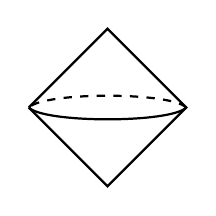
\begin{tikzpicture}[scale = 0.2, thick]
	\draw (5, 0) .. controls (4, -1) and (-4, -1) .. (-5, 0);
	\draw [dashed] (5, 0) .. controls (4, 1) and (-4, 1) .. (-5, 0);
	% \draw [dashed] (5, 0) arc [start angle = 0, delta angle = 180, x radius = 5.0cm, y radius = 1.0cm];
	\draw (-5, 0) -- (0, 5) -- (5, 0) -- (0, -5) -- (-5, 0);
\end{tikzpicture}
\captionsetup{font=footnotesize}
\caption{圆盘之悬垂}
\end{wrapfigure}
14. {\bf 悬垂}(suspension)\footnote{翻译参考日文\ruby[m]{懸垂}{けん|すい}}. 字面意思是将复形悬挂于两个固定点之间. 数学上的描述为, 复形 $X$ 的悬垂是将 $X \times I$ 中的 $X \times \{0\}$ 和 $X \times \{1\}$ 分别``缩''成一个点得到的商空间, 记作 $SX$. 右图是 $S^n$(中间的圆) 对应的 $S S^n$, 即从 $n$ 维圆的每个点向上下两个(极)点连结线段, 得到两个空心锥扣合而成的复形. 图中可以看出 $S S^n = S^{n + 1}$, 这也是因为上下两个锥都等同于 $e^n$, 而 $S^{n + 1}$ 可以看作两个 $e^{n + 1}$ 粘到 $S^{n}$ 得到的. 

悬垂是上下两个锥并起来, 那自然也可以只长出一个锥, 也就是:

15. {\bf 锥}(cone). 复形作底, 向上长出一个锥体. 也就是 $CX := X \times I / (X \times \{0\})$.

16. {\bf 连结}(join). 连结的概念可以从锥开始推广. 锥可以看作是从复形 $X$ 的每个点向一个特定的点连线段, 所有线段之并形成的复形. 而连结操作就是推广``特定的点''为一般的空间. 即如给定两个胞腔复形 $X$ 和 $Y$, 在它们的所有点对间连线, 其并形成的新复形称为 $X$ 和 $Y$ 的连结 $X \ast Y$. 或者用商空间的方法描述, 就是 $X \times Y \times I$ 的商, 等价关系是 $(x, y_1, 0) \sim (x, y_2, 0$ 及 $(x_1, y, 1) \sim (x_2, y, 1)$. 例如锥可以看作 $X \ast \cdot$, 和点的连结; 两条线段的连结可以形成一个四面体(如图 \ref{0-1::pic::join})

\begin{figure}[h]
\input{pictures/join-example.tikz}
\caption{两条线段的连结}
\end{figure}